% !TeX root = ../main.tex

\chapter{数值实验}

\section{算法测试结果}

\subsection{复现SVRG}

为保证对论文\inlinecite{johnsonAcceleratingStochasticGradient}的理解正确以及不遗漏技术细节,这里本文使用Julia编程语言复现了论文中对SVRG与SGD的性能测试。

所有测试中损失函数表达式均为
\begin{equation}\label{key}
P(w) = \frac1n \sum_{i=1}^n f_i(w)
\end{equation}
$f_i(w)$为随机生成的$w$的正定二次型,保证论文中强凸条件以及莱布尼兹连续条件被满足。

\begin{figure}[htb]
	\centering
	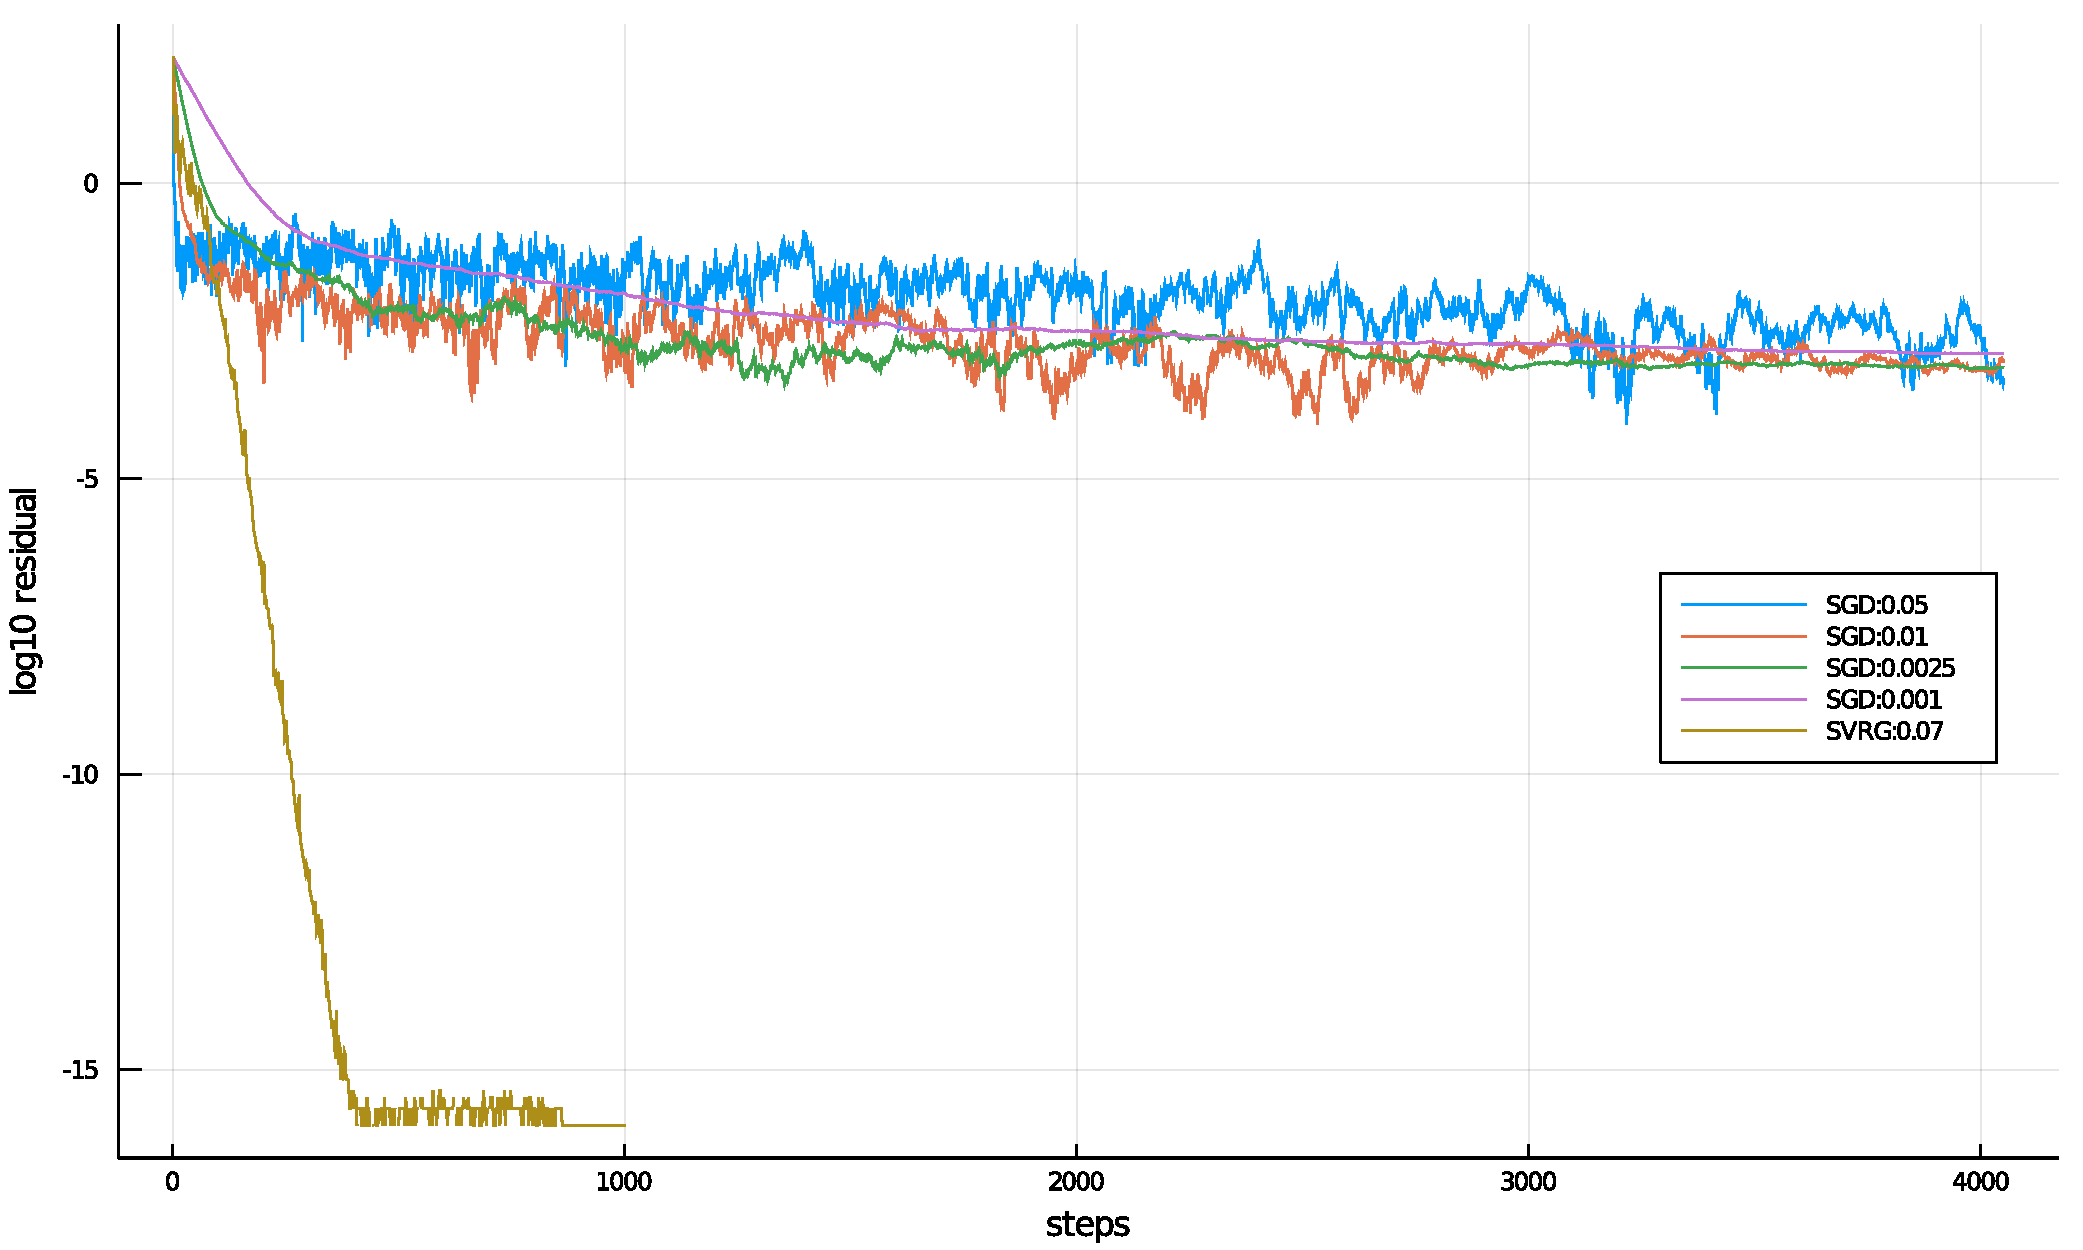
\includegraphics[width=1\textwidth]{image/sgd-vs-svrg.pdf}
	\caption{SGD与SVRG性能测试}
	\label{fig:sgd-svrg}
	\note{注:图中复现了SVRG原始论文中的算法性能比较\cite[7]{johnsonAcceleratingStochasticGradient},图例中前4条为SGD在最优学习速率附近不同值处的表现,最后一条为SVRG接近最优参数下的一个结果,数字表示步长(学习速率)。图中对SVRG数据的横坐标进行了$\frac{L_o+L_i m}{mL_\text{SGD}}\approx 1.25$的拉伸,保证相同横坐标下每一步平均使用的马尔科夫链长相等。}
\end{figure}
\begin{figure}[htb]
	\centering
	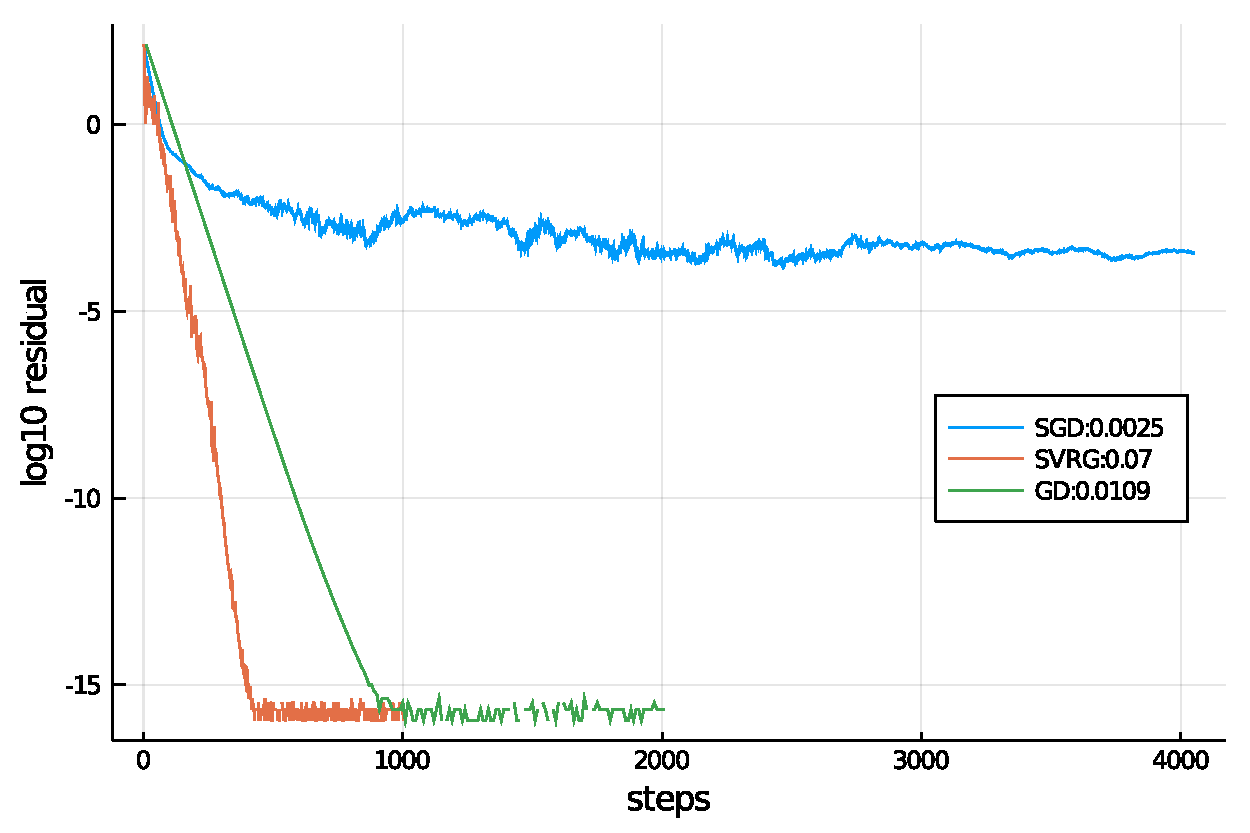
\includegraphics[width=1\textwidth]{image/sgd-vs-svrg2.pdf}
	\caption{SGD、SVRG与GD性能测试}
	\label{fig:sgd-svrg2}
	\note{注:接上图,加入了与常用无随机性梯度下降(GD)的比较,其横坐标被扩大了约1.25倍以保证相同横坐标下每一步平均使用的马尔科夫链长相等。等工作量下最佳SVRG优于最佳全梯度下降。}
\end{figure}

在图\ref{fig:sgd-svrg}中SVRG的表现远优于基础的SGD算法,且与原论文中测试结果一致,即论文中的SVRG在面对极值问题时的性能远优于随机梯度下降,且线性收敛。实验中,随机梯度下降为了保证结果的收敛,必须使步长随迭代次数$k$做$\mathcal{O}(1/k)$的缩小,并且结果的收敛速度在对数图中不断变慢。SVRG算法中步长始终是不变的,保证了对数图中常数下降速度,符合收敛速度$\mathcal{O}(\rho^k)$的理论预测。

\subsection{算法改造}

\begin{algorithm}[htb]
	\SetKwData{Left}{left}
	\SetKwData{This}{this}
	\SetKwData{Up}{up}
	\SetKwFunction{Union}{Union}
	\SetKwFunction{FindCompress}{FindCompress}
	\SetKwInOut{Input}{input}
	\SetKwInOut{Output}{output}
	
	\Input{待求问题$R=E$,更新频率$m$与学习速率$\eta$}
	\Output{末态$w^*$}
	
	初始化随机数,输入初态张量网络$\tilde{w}_0$\;
	\For{$s=1,2,\dots $}{
		$\tilde{w}=\tilde{w}_{s-1}$\;
		$\tilde{\mu} = \nabla R(\tilde{w})=\nabla\left(\frac1Z \sum_{S}W_{\tilde{w}}(S)^2 E(S)\right)$\;
		$w_0=\tilde{w}$\;
		由$\tilde{w}$生成马尔科夫链,样本集合为$\mathcal{L}$,样本数$\lvert \mathcal{L}\rvert = L_\text{outer}$\;
		\For{$t=1,2,\dots,m$}{
			选择一(SVRG1):无视$\mathcal{L}$,生成新马尔科夫链$\xi$使得$\lvert\xi\rvert=L_\text{inner}$\;
			选择二(SVRG2):随机选取$\xi\in\mathcal{L}$且$\lvert \xi \rvert=L_\text{inner}$\;
			利用公式(\ref{eq-gradient})计算样本$\xi$下能量梯度$\nabla\psi_{\xi}$的值\;
			$g_{t-1}=\nabla\psi_{\xi}(w_{t-1};\tilde{w})-\nabla\psi_{\xi}(\tilde{w}) + \tilde{\mu}$\;
			更新$w_t = w_{t-1}-\eta g_{t-1}$\;
		}
		$\tilde{w}_s=w_m$
	}
	\caption{马尔科夫链上的SVRG算法}
	\label{algo:algorithm3}
\end{algorithm}

张量网络的梯度优化法中的随机梯度下降与原始版本不同,加入了马尔科夫链上的重要抽样方法,因此我们将其改造为SVRG时也要做适当的改进,利用上一章中的reweighting方法,我们将SVRG与马尔科夫抽样方法结合,将算法\ref{algo:algorithm2}改造为算法\ref{algo:algorithm3}并测试其有效性。

\begin{figure}[htb]
	\centering
	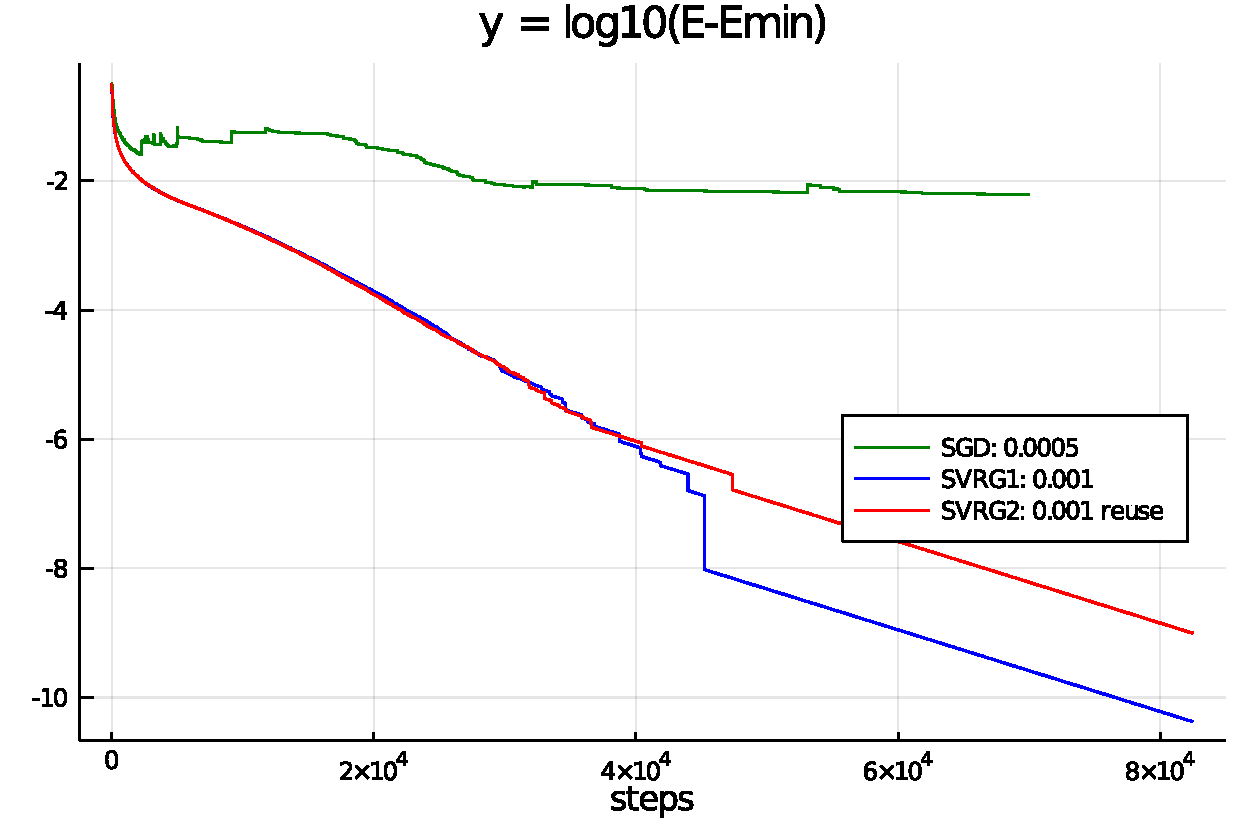
\includegraphics[width=\textwidth]{image/SVRGexTest3_d=20.pdf}
	\caption{SGD,SVRG测试$(d=20)$}
	\label{fig:sgd-svrg3}
	\note{注:横坐标为步长,SVRG的两条线分别代表算法\ref{algo:algorithm3}中两种选择,图例中数字为学习速率$\eta$}
\end{figure}

\begin{figure}[htb]
	\centering
	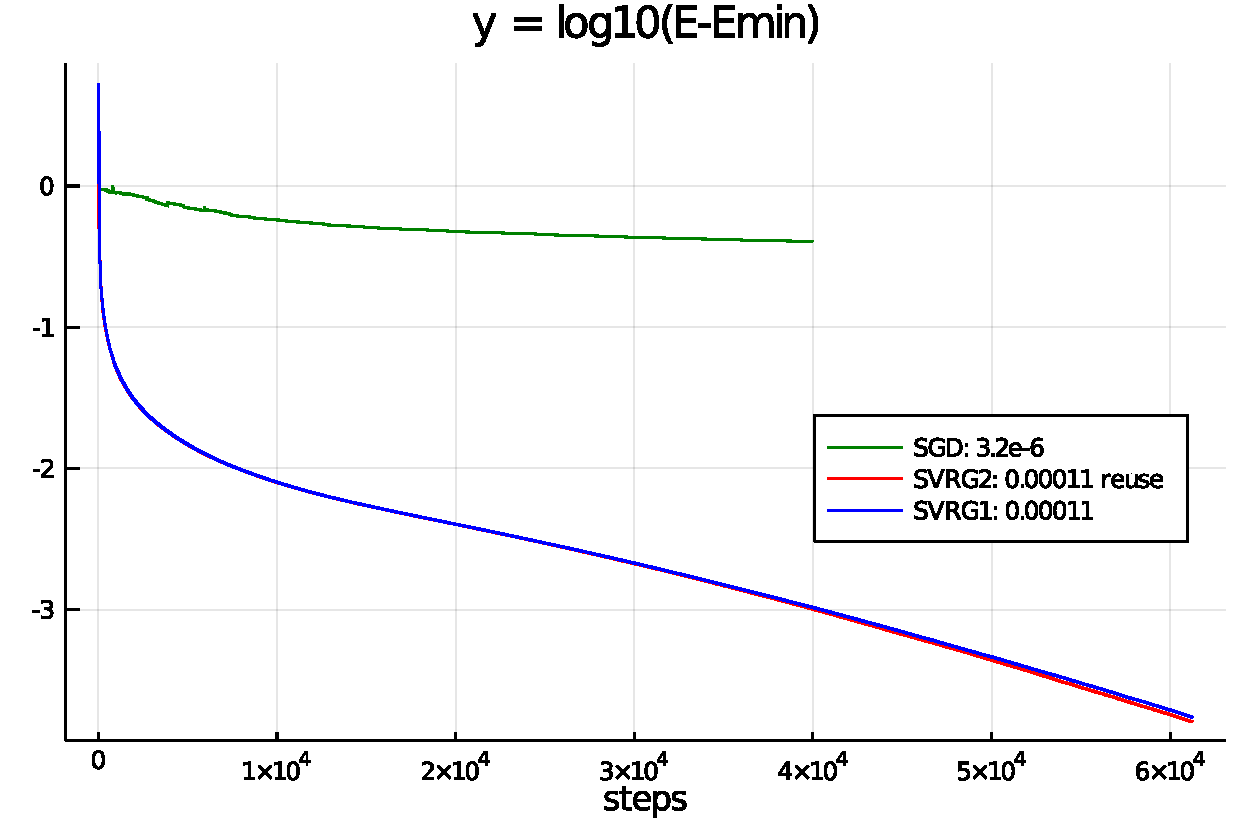
\includegraphics[width=\textwidth]{image/SVRGexTest1_d=200.pdf}
	\caption{SGD,SVRG测试$(d=200)$}
	\label{fig:sgd-svrg3-2}
	\note{注:增大态空间维度$d$. SVRG的两条线分别代表算法\ref{algo:algorithm3}中两种选择}
\end{figure}

与SGD相比,SVRG每一步的平均开销为$(L_\text{outer}+2mL_\text{inner})/{m}$,若SGD中使用的马尔科夫链长为$L$,则两种算法每走一步,其理想情况下计算开销之比为
\begin{equation}
\gamma = \frac{L_\text{outer}+2mL_\text{inner}}{mL}
\end{equation}
为了反映等工作量前提下两种算法的性能,本章所有数据涉及到SGD与SVRG的能量随步长变化曲线的,SVRG数据的横坐标均乘以$\gamma$以保证横坐标相同时其工作量与SGD一致。

为了避免在大规模服务器上做测试,本文采用了最简单的张量网络,即长度为1的MPS,只有一个一阶张量,回到了原始的$\ket{\varphi}=\sum c_i\ket{s_i}$的形式,利用最简单的计算验证新的SVRG算法是否可行。

结果如图\ref{fig:sgd-svrg3}所示,SVRG在开始时速度不稳定,迭代一定步数后变为平稳的$\mathcal{O}(\rho^k)$. 相比之下,普通的随机梯度下降速度越来越落后于SVRG。增大态空间维度,则使算法收敛的步长需要缩小,如图\ref{fig:sgd-svrg3-2}所示。即使加入了马尔科夫抽样与reweighting方法,SVRG缩减方差的原理依然成立,因此改造后的SVRG算法对于优化物理系统的能量极小值仍然可行。
\begin{figure}[htb]
	\centering
	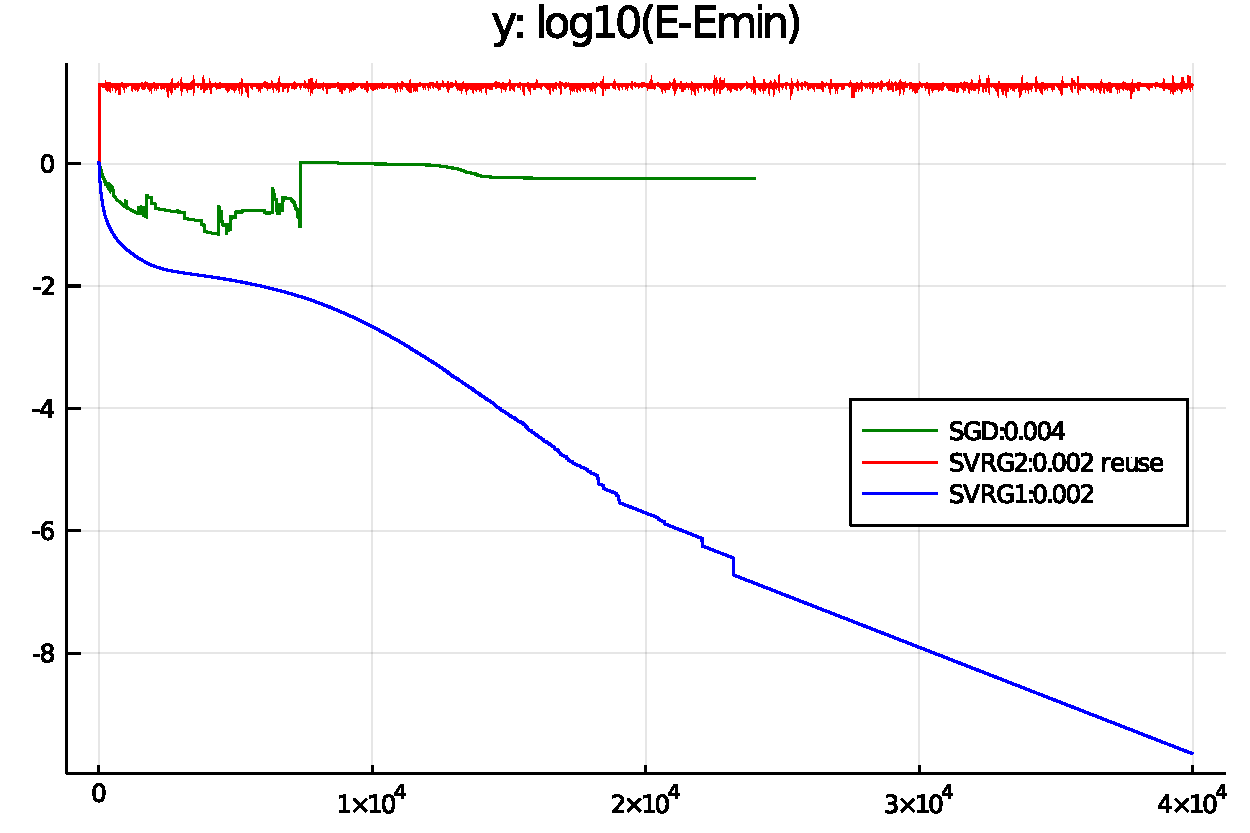
\includegraphics[width=1\textwidth]{image/SVRGexTest6_diverge.pdf}
	\caption{SGD,SVRG测试$(d=20)$}
	\label{fig:sgd-svrg4}
	\note{注:此图中的SGD与SVRG2陷入局域极小值}
\end{figure}

\section{结论与推广}

\subsection{结论}

前人通过改造SGD算法,使其能够使用至张量网络上,并取得了相当的成果。本文受方差缩减的随机梯度下降启发,尝试将普通SGD改造为SVRG的方法应用至张量网络的SGD上。在张量网络中采用SVRG之前,需要首先验证改造后算法的有效性,本文的数值实验中,SVRG在相当的迭代次数后表现为理论预测的$\mathcal{O}(\rho^k)$收敛,说明新的算法可以正确收敛至能量极小值,且是线性收敛的。这验证了被改造后算法的有效性,使人们能初步确定新的算法是一个正确的算法。

\subsection{算法推广}
\subsubsection{一般MPS}

正如前人将随机梯度下降结合马尔科夫链上的重要抽样方法应用于张量网络,我们将SVRG算法同样应用于张量网络。在SVRG中,如果不计算$\psi_{\xi}(w)$,即马尔科夫链长为零,则我们的算法退化为全梯度下降;如果不计历史梯度$R(\tilde{w})$与$\psi_{\xi}(\tilde{w})$则退化为随机梯度下降。我们做出推测,SVRG在长度不为一的MPS上,应该与SGD或全梯度下降在其上一样有效。同样的,SVRG也继承了原先算法的缺点,即应使用一个接近基态的初态进行优化,比如由虚时演化得到的近似基态\cite{liuGradientOptimizationFinite2017},否则容易如图\ref{fig:sgd-svrg4}陷入局域极小值中。

\subsubsection{推广至PEPS}

由于PEPS与MPS中一个显著的不同便是PEPS的精确缩并时间复杂度是指数级的,而近似缩并仍然有很高的时间复杂度,因此我们无法断定SVRG在PEPS中一样有效,因为随着斯通的增大,计算一步全梯度$R(w)$的开销可能会远大于方差缩减节省的开销。我们需要更多的数值实验来研究其在PEPS上的有效性。
